\documentclass[12pt, a4paper, UTF8]{ctexart}

\usepackage{UCASReport}
\usepackage{bm}
\usepackage{tikz}
\usepackage{float}
\usepackage{setspace}
\usepackage{enumitem}
\usepackage{booktabs}
\usepackage{listings}
\usepackage{amsmath, amssymb, amsfonts}
\usepackage[table]{xcolor}

\setlist[1]{
    itemsep = 0pt,
    partopsep = 0pt,
    parsep = 0pt,
    topsep = 5pt,
    leftmargin = 2em,
    labelsep = 0.25em
}

\definecolor{codegreen}{rgb}{0, 0.6, 0}
\definecolor{codegray}{rgb}{0.5, 0.5, 0.5}
\definecolor{codepurple}{rgb}{0.58, 0, 0.82}
\definecolor{backcolour}{rgb}{0.95, 0.95, 0.92}
\definecolor{MorandiLightCyan}{RGB}{209, 238, 238}
\definecolor{MorandiBlue}{RGB}{70, 110, 255}
\definecolor{MorandiGrey}{RGB}{80, 100, 100}
\definecolor{MorandiRed}{RGB}{220, 130, 130}
\definecolor{MorandiOrange}{RGB}{250, 210, 160}

\lstset{
    backgroundcolor = \color{backcolour},
    commentstyle = \color{codegreen},
    keywordstyle = \color{magenta},
    numberstyle = \tiny\color{codegray},
    stringstyle = \color{codepurple},
    basicstyle = \ttfamily\footnotesize,
    breakatwhitespace = false,
    breaklines = true,
    captionpos = b,
    keepspaces = true,
    numbers = left,
    numbersep = 5pt,
    showspaces = false,
    showstringspaces = false,
    showtabs = false,
    tabsize = 2
}

\newcommand{\diff}[2]{\dfrac{\mathrm{d}#1}{\mathrm{d}#2}}
\newcommand{\diffn}[3]{\dfrac{\mathrm{d}^{#3}#1}{\mathrm{d}#2^{#3}}}
\newcommand{\piff}[2]{\dfrac{\partial{#1}}{\partial{#2}}}
\newcommand{\eval}[2]{\left.#1\right|_{#2}}
\newcommand{\e}{\mathrm{e}}
\renewcommand{\d}{\mathrm{d}}
\newcommand{\barline}[1]{\overline{#1\rule{0pt}{1.5ex}}}
\newcommand{\mathsize}{\fontsize{6.5pt}{10pt}\selectfont}

\newcommand{\cube}[1]{
    \begin{tikzpicture}[baseline = 0ex]
        \draw[
            draw = #1,
            fill = #1!20,
            thick,
            rounded corners = 0.5pt
        ] (0,0) rectangle (0.25, 0.25);
    \end{tikzpicture}
}



\begin{document}

\cover
\thispagestyle{empty}
\clearpage
\begin{spacing}{1.5}
    \tableofcontents
\end{spacing}
\clearpage



\section{竞赛背景}
\subsection{问题描述}
本报告基于 Kaggle 竞赛的“Natural Language Processing with Disaster Tweets”，该任务的核心目标是构建一个机器学习模型，用于判断 Twitter 上的推文是否在描述真实的灾难性事件，这是一个典型的二分类自然语言处理问题。

在紧急情况下，Twitter 已成为重要的沟通渠道，智能手机的普及使得人们能够实时发布他们观察到的紧急情况，正因如此，越来越多的机构，譬如救灾组织和新闻机构，开始对 Twitter 进行程序化监控。单词“Ablaze”，既可以表示着火也可以表示情绪高涨，这样的词汇可以描述字面上的火灾，也可以隐喻地描述某种热烈的氛围。

数据集包含三个主要字段：

\begin{itemize}
    \item \textbf{text}：推文的具体文本内容；
    \item \textbf{keyword}：推文中包含的特定关键词，注意可能为空；
    \item \textbf{location}：推文发出的地点，注意也可能为空；
    \item \textbf{target}：标签，其中 1 代表真实灾难，0 代表非灾难。
\end{itemize}



\subsection{建模思路}
观察数据集注意到推文长度通常较短，平均词数较低，导致传统统计特征表达能力有限，需要上下文建模能力较强的模型，因此我们小组考虑本竞赛采用了从基础统计分析到深度学习微调的渐进式建模思路，具体流程如下：

\begin{enumerate}
    \item \textbf{探索性数据分析}：分析数据规模、缺失值、数据分布以及类别平衡性等信息；
    \item \textbf{数据清理与增强}：利用正则表达式处理噪声，并将 keyword 和 location 信息融合进入 text 作为输入；
    \item \textbf{Baseline 模型}：利用 TF-IDF 和逻辑回归建模，作为基线模型；
    \item \textbf{提升模型}：使用传统的机器学习算法，例如决策树、支持向量机、朴素贝叶斯等算法进行效果提升试验；
    \item \textbf{BERT 微调}：使用预训练的 Bert-Large-Uncased 模型，通过迁移学习提取深层语义特征；
    \item \textbf{AdaBoost 集成学习}：通过将传统的机器学习与 BERT 模型集成，进行集成训练；
    \item \textbf{模型评估}：通过评估预测答案与期望答案之间的 $F_1$ 得分\autoref{eq-s}，选取最优结果。
\end{enumerate}

\begin{equation}
    F_1=2\ast\dfrac{\text{Precision}\ast\text{Recall}}{\text{Precision}+\text{Recall}} \label{eq-s}
\end{equation}

其中：

\begin{equation}
    \begin{cases}
        \text{Precision}=\dfrac{\text{TP}}{\text{TP}+\text{FP}}
        \\[10pt]
        \text{Recall}=\dfrac{\text{TP}}{\text{TP}+\text{FN}}
    \end{cases}
\end{equation}

最终项目需要逐步构建一个能够理解上下文语义、抵抗文本噪声、利用辅助字段信息、处理短文本数据的稳健二分类模型。



\section{探索性数据分析}
在进行模型训练之前，首先对训练集和测试集进行了详细的统计分析，代码中实现了 \verb|statistics()| 函数，用于监控数据的基本特征。



\subsection{数据规模与内存占用}

\begin{itemize}
    \item \textbf{训练集 Train}：包含约 7613 条样本，用于模型的参数更新；
    \item \textbf{测试集 Test}：包含约 3263 条样本，用于生成最终提交结果。
\end{itemize}

通过 Pandas 库的 \verb|memory_usage()| 函数，监控了数据加载的内存占用情况，其中训练集大小 200KB，测试集大小 82KB，确保在有限的计算资源下，如 GPU、RAM 显存内存限制，能够高效处理数据。结果表明，数据体量极小，I/O 并不是性能瓶颈，GPU 显存主要用于模型而非数据，因此可安全进行多轮 Epoch 迭代训练，并且增加 Batch Size 提升吞吐率。



\subsection{缺失值分布}
数据中存在显著的缺失值问题，集中在 keyword 和 location 维度列。其中 keyword 缺失率相对较低，这部分信息对于区分特定类型的灾难，譬如 flood、fire 具有重要指示意义，location 缺失率较高，且非结构化严重，然而尽管如此，地点信息对于判断灾难的真实性具有辅助作用。

代码通过以下逻辑计算缺失分布：

\begin{lstlisting}[language = Python]
missing_columns = ['keyword', 'location']
missing_distribution = df[missing_columns].isnull().sum()
print(f'{label}缺失值:')
print(f"keyword = {missing_distribution['keyword']}", end = '')
print(f"({(100 * missing_distribution['keyword'] / df.shape[0]):.3f}%)")
print(f"location = {missing_distribution['location']}", end = '')
print(f"({(100 * missing_distribution['location'] / df.shape[0]):.3f}%)")
\end{lstlisting}

这种分析指导了我们在后续预处理中，对于缺失值采用了填补空字符串的策略，而不是直接丢弃样本。最终结果表明，训练集 keyword 缺失值有 61 个，location 缺失值有 2533 个，测试集 keyword 缺失值有 26 个，location 缺失值有 1105 个，训练集 keyword 类型数有 221 个，location 类型数有 3341 个，测试集 keyword 类型数有 221 个，location 类型数有 1602 个。由于 location 占比例极大，噪声严重且长尾分布明显，因此可以从缺失值数量以及类型数量忽略部分该维度不重要的样本，尽量保留信息集中且结构化的 keyword 维度用于分析。



\section{文本清洗}
由于 Twitter 文本中包含大量 Emoji 非正式用语、HTML 的 \verb|#| 标签、用户 \verb|@| 提及和 URL 链接，直接输入模型会引入大量噪声，在 Python 主函数中实现专门的 \verb|regex()| 函数和文本构造逻辑。



\subsection{正则化表达式清洗}
为了规范化文本，我们小组定义了以下清洗规则：

\begin{itemize}
    \item \textbf{URL 替换}：Twitter 中的链接通常是 \verb|http://t.co/...| 格式，这些随机字符对语义理解没有帮助，但链接的存在本身可能暗示这是一种新闻报道，因此将所有链接统一替换为特殊标记 \verb|<URL>|；
    \item \textbf{用户 @ 提及替换}：将 \verb|@username| 替换为 \verb|<USER>|，以去除具体用户名的干扰，同时保留“有人被提及”这一结构信息；
    \item \textbf{HashTag 处理}：移除 \verb|#tag| 符号但保留标签文本内容，因为标签内容往往是句子的核心语义；
    \item \textbf{空白字符标准化}：将多余的空格、换行符替换为单个空格。
\end{itemize}



\subsection{特征融合策略}
不同于传统的将 keyword 和 location 进行 One-Hot 独热编码单独处理，利用 LLM 强大的上下文理解能力，将这两个特征显式拼接到输入文本中。构造后的输入格式为：
\begin{equation}
    \text{input}=\texttt{"}[\text{keyword}: K]\quad[\text{location}: L]\quad T\texttt{"}
\end{equation}

其中 $K$ 是关键词，$L$ 是地点，$T$ 是清洗后的推文内容，若 $K$ 或 $L$ 缺失，则该部分为空。这种 Prompt Engineering 处理方式使得模型能够学习到：当 location 存在时，文本描述灾难的可能性是否更高，或者特定的 keyword 与特定的上下文结合时，其语义倾向如何变换，代码在 \verb|generate()| 函数中实现了这一逻辑，并将处理后的数据保存。



\section{Baseline}\label{sec:baseline}
我们首先使用 TF-IDF 文档向量化的方式获取训练数据的向量化表示，随后使用 Logistic Regression 分类算法作为本次实验的基线标准。



\subsection{TF-IDF 文档向量化}
TF-IDF（Term Frequency–Inverse Document Frequency）是一种用于衡量词语在文档中重要程度的统计方法，广泛应用于信息检索与文本挖掘领域。其基本思想是：一个词语对某篇文档的重要性，既取决于它在该文档中出现的频率，也受到它在整个语料库中分布广度的影响。具体而言，如果一个词在某文档中频繁出现，同时在其他文档中很少出现，则该词对该文档具有较高的区分能力，其TF-IDF值也相应较高。

TF-IDF由两部分构成：词频（Term Frequency, TF）和逆文档频率（Inverse Document Frequency, IDF）。词频反映词语在单篇文档中的出现次数，通常采用归一化形式以消除文档长度差异带来的偏差；逆文档频率则刻画词语在整个语料库中的稀有程度，通过取文档总数与包含该词的文档数之比的对数来计算。将两者相乘，即可得到该词在特定文档中的TF-IDF权重。这一权重能够有效抑制常见停用词的影响，同时突出具有代表性的关键词。

具体而言，词语的词频具有如下定义：
$$
\mathrm{TF}(t, d) = \frac{N(t)}{N(d)}
$$
其中 $N(t)$ 为词语 $t$ 在文档 $d$ 中出现的次数，$N(d)$ 为文档 $d$ 的总词数。逆文档频率定义如下：
$$
\mathrm{IDF}(t,D) = \log \frac{N}{\mathrm{df}(t)}
$$
其中 $N$ 为语料库中的总文档数，$\mathrm{df}(t)$ 为在所有文档中出现词语 $t$ 的文档数。为了防止除以零，一般也会对该式进行拉普拉斯平滑操作，如 $\mathrm{IDF}(t,D)=\log \frac{N+1}{\mathrm{df}(t)+1}$。通过以上定义，TF-IDF 便可以定义为：
$$
\text{TF-IDF}(t, d, D) = \mathrm{TF}(t, d) \times \mathrm{IDF}(t, D)
$$
该值越大，说明词语 $t$ 对文档 $d$ 越有代表性。

% 需要注意的是，TF-IDF本身并不涉及文本的分词过程，而是在文本已经完成分词和预处理（如去除停用词、统一大小写等）的基础上进行的特征加权步骤。因此，在实际应用中，尤其是处理中文文本时，必须首先借助分词工具将原始句子切分为词语序列，然后才能构建词袋模型并计算TF-IDF值。最终，每篇文档可被表示为一个高维向量，其中每一维对应词表中的一个词，其数值即为该词的TF-IDF权重，这种向量表示可直接用于文本分类、聚类、相似度计算等下游任务。

% 尽管TF-IDF方法简洁高效，并在许多传统自然语言处理任务中表现良好，但它基于词袋假设，忽略了词语的顺序、语法结构及深层语义信息，因而在处理复杂语义或短文本时存在一定局限。随着深度学习的发展，词嵌入和预训练语言模型逐渐成为主流，但TF-IDF因其可解释性强、计算效率高，仍在诸多实际场景中具有重要价值。

TF-IDF 可以用于文档的向量化。首先将每篇文档（对应训练数据的每条数据点中包含的语句）经过分词处理，得到所有文档集合的词表（vocabulary），最终为 $\forall d\in D$ 计算对应的 $\text{TF-IDF}(\boldsymbol{t}, d, D)$ 向量（其中 $\boldsymbol{t}$ 为分词后的词表向量）即得到了每篇文档的向量化表示。



\subsection{Logistic Regression 对数几率回归}
对数几率回归（逻辑回归）是一种广泛应用于分类问题的统计学习方法，尤其适用于二分类任务。尽管其名称中含有「回归」二字，但其本质是一个分类模型。其核心思想在于：通过 Sigmoid 函数的非线性变换，将线性回归模型的连续值输出映射到介于 0 和 1 之间的概率值，从而实现对样本属于某一类别的概率进行建模。具体而言，给定一个特征向量 $x$，逻辑回归模型假设其属于正类（通常标记为 $1$）的概率 $P(y=1|\boldsymbol{x})$ 由以下公式表示：
$$P(y=1|\boldsymbol{x}) = \frac{1}{1+e^{-\boldsymbol{w}^{\top}\boldsymbol{x} + b}}$$
其中，$\boldsymbol{w}$ 是权重向量，$b$ 是偏置项，$\boldsymbol{w}^{\top}\boldsymbol{x}+b$ 构成了一个线性决策函数。

模型训练的目标是找到最优的参数 $\boldsymbol{w}$ 和 $b$，使得模型预测的概率分布与数据的真实标签尽可能一致。这一过程通常通过最大似然估计来实现：
$$
\max_{\boldsymbol{w}} L(\boldsymbol{w}) = \prod_{i=1}^{N} p(y=1|\boldsymbol{x}_{i})^{y_{i}} \cdot [1-p(y=1|\boldsymbol{x}_{i})]^{1-y_{i}}
$$
上式取负对数得：
$$
\min_{\boldsymbol{w}} -\log L(\boldsymbol{w}) = -\sum_{i=1}^{N}y_{i}p_{i} + (1-y_{i}) (1-p_{i})
$$
其中 $p_{i}=p(y=1|\boldsymbol{x}_{i})$ 是模型预测的正类概率，$y_{i}$ 是真实标签（$0$ 或 $1$）。为了最小化损失函数并求解参数，通常采用梯度下降等优化算法进行迭代更新。

逻辑回归模型具有多个重要特性。首先，它直接输出具有良好统计解释的概率值，这对于需要概率评估的决策场景（如风险评估）非常有用。其次，其决策边界是由线性函数 $\boldsymbol{w}^{\top} \boldsymbol{x} + b=0$ 定义的一个超平面，这意味着它是一个线性分类器。虽然模型本身是线性的，但通过引入特征的多项式项或交互项等特征工程手段，可以间接地处理非线性可分的模式。此外，逻辑回归模型在训练完成后，可以通过分析权重系数 $\boldsymbol{w}$ 的大小和符号来对特征的重要性进行一定程度的解释，这是其相较于许多复杂「黑箱」模型的一个显著优势。



\subsection{实验结果}
在实验中，经过集中测试 TF-IDF 的超参数（调参过程见表~\ref{tab:tfidf-selection}），最终使用下述超参设置：

\lstset{
 columns=fixed,       
 numbers=left,                                        % 在左侧显示行号
 numberstyle=\tiny\color{gray},                       % 设定行号格式
 frame=none,                                          % 不显示背景边框
 backgroundcolor=\color[RGB]{245,245,244},            % 设定背景颜色
 keywordstyle=\color[RGB]{40,40,255},                 % 设定关键字颜色
 numberstyle=\footnotesize\color{darkgray},           
 commentstyle=\it\color[RGB]{0,96,96},                % 设置代码注释的格式
 stringstyle=\rmfamily\slshape\color[RGB]{128,0,0},   % 设置字符串格式
 showstringspaces=false,                              % 不显示字符串中的空格
 language=Python,                                        % 设置语言
}

\begin{small}
\begin{lstlisting}
TfidfVectorizer(
    max_features=2500,
    min_df=5,
    max_df=0.7,
    ngram_range=(1, 1),
    stop_words='english'
)
LogisticRegression(
    random_state=42,
    max_iter=1000,
    C=1.0
)
\end{lstlisting}
\end{small}

在上述超参设置下，最终结果如图~\ref{fig:baseline-logreg-result} 所示。

\begin{table}[H]
\centering
\begin{tabular}{c|cccc}
\toprule
\textbf{超参数设置} & \textbf{5000} & \textbf{2500} & \textbf{1200} & \textbf{600} \\ \midrule
\textbf{(1, 1)} & 0.7246 & \textbf{0.7276} & 0.7106 & 0.7061 \\
\textbf{(1, 2)} & 0.7164 & 0.7065 & 0.7083 & 0.7018 \\ \bottomrule
\end{tabular}
\caption{TF-IDF 不同的超参数配置产生的不同验证集 F1-Score。第一行表示使用的不同\textit{最大特征数}，第一列表示使用的不同 \textit{n-gram 范围}。}
\label{tab:tfidf-selection}
\end{table}

\begin{figure}
    \centering
    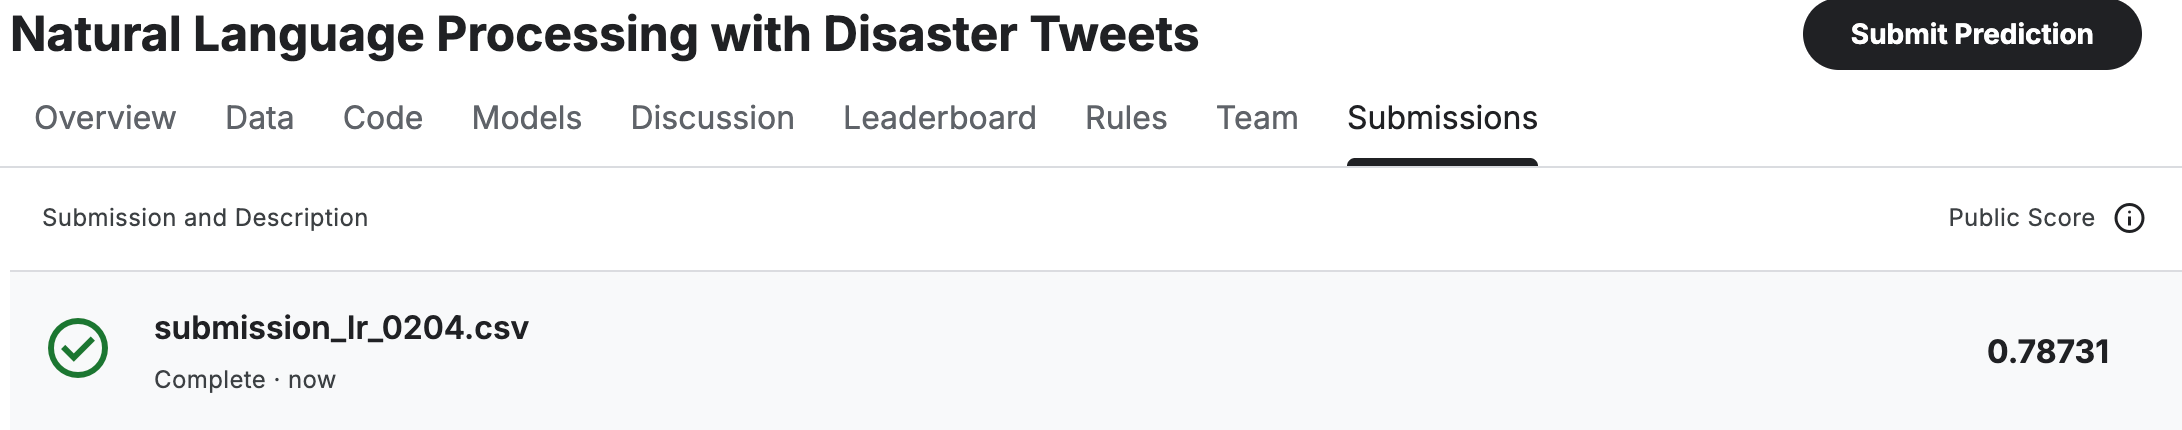
\includegraphics[width=0.85\linewidth]{./figs/logreg_result.png}
    \caption{TF-IDF + Logistic Regression 的基本结果}
    \label{fig:baseline-logreg-result}
\end{figure}

对数几率回归模型取得了 0.78731 的 F1-Score，为本次实验建立了坚实的性能基线。该结果充分表明，经过向量化的推特文本数据具有显著的线性可分特性。作为一种高效的广义线性模型，逻辑回归能够很好地适应文本分类任务中典型的高维稀疏特征空间，其通过正则化学习到的特征权重具有明确的解释性，同时模型输出的校准概率也为决策提供了可靠的置信度依据。这一基线分数说明，一个设计良好的线性分类器在此任务上已具备相当竞争力。



\section{提升模型}
本部分我们将在第~\ref{sec:baseline}~节的基线结果基础上，进一步探索更高级的线性分类方法（\ref{sec:enhancement-svm}~节线性核 SVM）以及非线性分类方法（\ref{sec:enhancement-svm}~节非线性核 SVM，\ref{sec:enhancement-decisiontree}~节决策树）和生成式方法（\ref{sec:enhancement-bayes}~节贝叶斯方法）在该问题上的表现。



\subsection{支持向量机（SVM）}\label{sec:enhancement-svm}
支持向量机（Support Vector Machine, SVM）是一种基于统计学习理论的监督学习模型，其核心思想是通过构建一个最优超平面来实现分类或回归任务。对于线性可分数据集，SVM的目标是找到一个分离超平面，使得两类样本之间的间隔最大化。设训练数据集为 $\{(\mathbf{x}_i, y_i)\}_{i=1}^n$，其中 $\mathbf{x}_i \in \mathbb{R}^d$，$y_i \in \{-1, +1\}$，分离超平面可表示为 $\mathbf{w}^\top \mathbf{x} + b = 0$。SVM的优化问题可形式化为以下凸二次规划问题：

\[
\begin{aligned}
\min_{\mathbf{w}, b} \quad & \frac{1}{2} \|\mathbf{w}\|^2 \\
\text{s.t.} \quad & y_i(\mathbf{w}^\top \mathbf{x}_i + b) \geq 1, \quad i = 1, \dots, n
\end{aligned}
\]

对于非线性可分情况，SVM引入松弛变量 $\xi_i$ 和惩罚参数 $C$，允许部分样本被错误分类，此时优化问题变为：

\[
\begin{aligned}
\min_{\mathbf{w}, b, \boldsymbol{\xi}} \quad & \frac{1}{2} \|\mathbf{w}\|^2 + C \sum_{i=1}^n \xi_i \\
\text{s.t.} \quad & y_i(\mathbf{w}^\top \mathbf{x}_i + b) \geq 1 - \xi_i, \\
& \xi_i \geq 0, \quad i = 1, \dots, n
\end{aligned}
\]

通过拉格朗日对偶变换，上述问题可转化为对偶问题，并引入核函数 $K(\mathbf{x}_i, \mathbf{x}_j) = \phi(\mathbf{x}_i)^\top \phi(\mathbf{x}_j)$ 将原始特征映射到高维空间，从而处理非线性可分问题。常用的核函数包括线性核、多项式核、径向基函数（RBF）核和Sigmoid核。SVM的决策函数为：

\[
f(\mathbf{x}) = \operatorname{sign}\left( \sum_{i=1}^n \alpha_i y_i K(\mathbf{x}_i, \mathbf{x}) + b \right)
\]

其中 $\alpha_i$ 为拉格朗日乘子，对应于支持向量。SVM通过结构风险最小化原则，在保证分类准确性的同时最大化分类间隔，具有良好的泛化能力。



\subsection{决策树}\label{sec:enhancement-decisiontree}
决策树（Decision Tree）是一种基于树结构的分类与回归模型，通过递归地划分特征空间构建决策规则。决策树的构建包括特征选择、树的生成和剪枝三个主要步骤。对于分类任务，常用的决策树算法包括ID3、C4.5和CART；对于回归任务，则主要采用CART算法。

特征选择的目标是选取对训练数据具有最强分类能力的特征。ID3算法使用信息增益作为特征选择准则，设训练数据集 $D$ 的类别集合为 $\mathcal{C} = \{c_1, \dots, c_k\}$，特征 $A$ 的信息增益定义为：

\[
\operatorname{Gain}(D, A) = \operatorname{Entropy}(D) - \sum_{v=1}^V \frac{|D^v|}{|D|} \operatorname{Entropy}(D^v)
\]

其中 $\operatorname{Entropy}(D) = -\sum_{i=1}^k p_i \log_2 p_i$ 为数据集 $D$ 的经验熵，$p_i$ 为类别 $c_i$ 在 $D$ 中的比例，$V$ 为特征 $A$ 的取值个数，$D^v$ 为 $A$ 取第 $v$ 个值的子集。C4.5算法使用信息增益比来修正信息增益对取值较多特征的偏好：

\[
\operatorname{GainRatio}(D, A) = \frac{\operatorname{Gain}(D, A)}{\operatorname{IV}(A)}, \quad \operatorname{IV}(A) = -\sum_{v=1}^V \frac{|D^v|}{|D|} \log_2 \frac{|D^v|}{|D|}
\]

CART算法对于分类任务使用基尼指数作为特征选择准则，对于回归任务则采用平方误差最小化准则。决策树的生成通过递归地选择最优特征进行数据划分，直到满足停止条件（如节点样本数低于阈值或所有样本属于同一类别）。为防止过拟合，决策树需要进行剪枝，包括预剪枝和后剪枝两种策略。预剪枝在生成过程中提前停止树的生长，后剪枝则在生成完整决策树后通过验证集剪除冗余分支。



\subsection{贝叶斯模型}\label{sec:enhancement-bayes}
贝叶斯模型基于贝叶斯定理构建，通过结合先验概率和样本数据计算后验概率，从而实现分类与推理。朴素贝叶斯分类器是贝叶斯模型中最常用的方法，其假设特征之间条件独立，即给定类别 $c$ 时，特征 $\mathbf{x} = (x_1, \dots, x_d)$ 满足：

\[
P(\mathbf{x} \mid c) = \prod_{j=1}^d P(x_j \mid c)
\]

对于类别 $c$，朴素贝叶斯分类器通过最大化后验概率进行分类：

\[
\hat{c} = \arg\max_{c \in \mathcal{C}} P(c \mid \mathbf{x}) = \arg\max_{c \in \mathcal{C}} P(c) \prod_{j=1}^d P(x_j \mid c)
\]

其中 $P(c)$ 为类别的先验概率，可通过训练数据估计。对于连续特征，通常假设其服从高斯分布，并通过最大似然估计计算均值和方差；对于离散特征，则直接计算各类别下特征取值的频率。

贝叶斯网络（Bayesian Network）是更一般的贝叶斯模型，通过有向无环图表示变量之间的依赖关系。设变量集合为 $\mathbf{X} = \{X_1, \dots, X_n\}$，贝叶斯网络联合概率分布可分解为：

\[
P(X_1, \dots, X_n) = \prod_{i=1}^n P(X_i \mid \operatorname{Pa}(X_i))
\]

其中 $\operatorname{Pa}(X_i)$ 表示 $X_i$ 的父节点集合。贝叶斯网络的学习包括结构学习和参数学习两部分：结构学习旨在从数据中推断网络拓扑，常用方法包括基于约束的方法和基于评分的方法；参数学习则在给定网络结构下估计条件概率分布。

贝叶斯模型通过引入先验知识，能够有效处理小样本问题，并提供概率形式的输出，适用于不确定性推理。然而，朴素贝叶斯的条件独立假设在实际问题中往往过于严格，贝叶斯网络则通过建模变量间的依赖关系提供了更灵活的框架。



\subsection{实验结果}
在接下来的实验中，我们依旧采取与第~\ref{sec:baseline}~节中相同的文本向量化方式，即使用 TF-IDF 向量化，并且根据每种模型的验证效果，稍微调最大特征数以及 n-gram 范围两项超参数设置。



\subsubsection{线性核 SVM}
在线性核 SVM 中，核函数 $K(\boldsymbol{x}_i, \boldsymbol{x}_j)$ 使用简单的线性函数，如向量内积 $K(\boldsymbol{x}_i, \boldsymbol{x}_j)=\boldsymbol{x}_i^{\top} \boldsymbol{x}_j$。在本实验中我们即采用向量内积作为线性核。SVM 惩罚系数 $C$ 设置为 1。经过验证集实验，TF-IDF 的最大特征数为 600，n-gram 范围为 $(1, 1)$。实验结果如图~\ref{fig:enhancement-linearsvm-result} 所示。

线性核 SVM 取得了 0.77995 的 F1 分数，与多数几率回归性能极为接近。这一微小差异可能源于两种模型优化目标的不同：线性 SVM 聚焦于边界样本（支持向量）以最大化间隔，而逻辑回归则考虑所有样本的似然概率进行参数估计。两者性能处于同一梯队，再次强有力地证实了数据中存在的核心线性模式。软间隔机制的引入使模型能够容忍个别噪声或异常样本，从而获得一个更具泛化能力的鲁棒线性超平面，这正是在实际文本分类任务中所需要的。



\subsubsection{非线性核 SVM}
实验中，我们采用了 RBF 核作为核函数。RBF 核定义如下：
$$
K(\boldsymbol{x}_i, \boldsymbol{x}_j) = \exp \left( \gamma \cdot \mathrm{Dist}(\boldsymbol{x}_i, \boldsymbol{x}_j) \right)
$$
在代码实现中，我们使用 $\gamma$ 的默认参数设置（\verb|'scale'|），以及使用 L2 距离作为 $\mathrm{Dist(\cdot, \cdot)}$ 函数。TF-IDF 的最大特征数为 1100，n-gram 范围为 $(1,1)$。实验结果如图~\ref{fig:enhancement-rbfsvm-result} 所示。

使用 RBF 核的支持向量机取得了本次实验中目前最优的性能，F1 分数达到 0.7919。这一结果揭示了数据中除主体线性结构外，还存在一些非线性可分模式。RBF 核通过将样本映射到高维特征空间，能够捕捉词语之间更复杂的交互关系与局部语境模式，这些可能是单纯线性加权无法完美表征的。值得关注的是，其性能提升幅度虽显著但有限，这表明数据中的非线性模式是对主要线性趋势的补充与修正，而非主导。该结果也展示了非线性 SVM 能在控制过拟合风险的前提下，有效挖掘并利用这些复杂模式。

\begin{figure}[H]
    \centering
    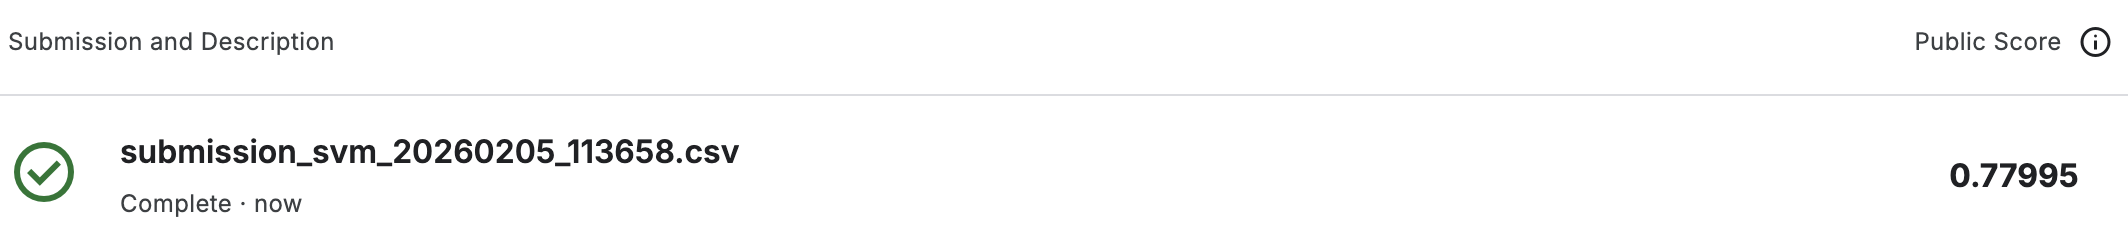
\includegraphics[width=0.85\linewidth]{./figs/svm-result_2026-02-05_11-38-35.png}
    \caption{线性核 SVM 的实验结果}
    \label{fig:enhancement-linearsvm-result}
\end{figure}

\begin{figure}[H]
    \centering
    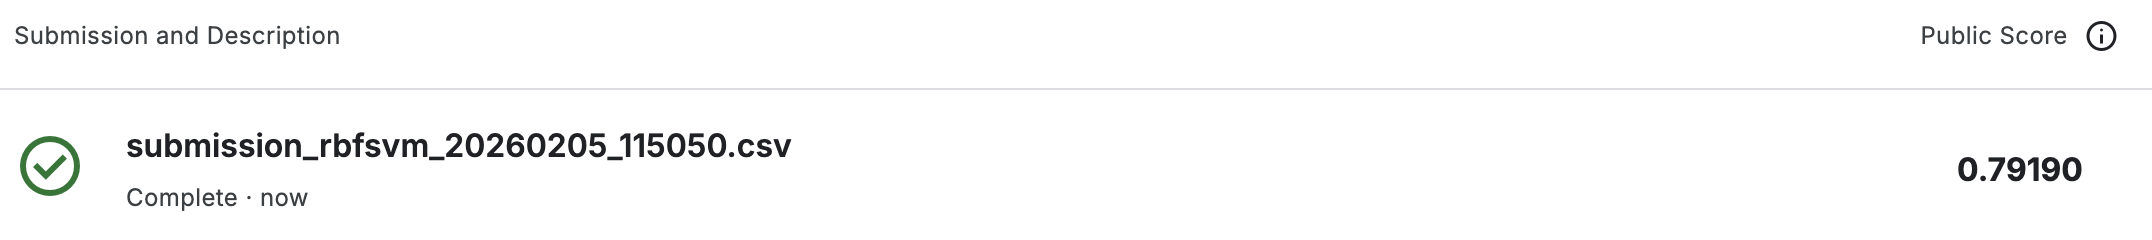
\includegraphics[width=0.85\linewidth]{./figs/rbfsvm-result_2026-02-05_11-51-39.png}
    \caption{RBF 核 SVM 的实验结果}
    \label{fig:enhancement-rbfsvm-result}
\end{figure}



\subsubsection{决策树}
实验中我们采用 Gini 指数以及树节点二分法（CART）的决策树。不限制树的最大深度，并规定树的非叶节点最少需要有 2 个样本才能进行分裂，叶节点最少需要有 1 个样本。TF-IDF 最大特征数为 2500，n-gram 范围为 $(1,1)$。实验结果如图~\ref{fig:enhancement-dectree} 所示。

决策树模型的表现不尽如人意，其 0.70027 的 F1 分数显著落后于其他模型。我们将此归因于源于模型假设与数据特性之间的根本性不匹配。决策树依赖基于单个特征阈值的递归分割机制，而在文本分类形成的高维、稀疏特征空间中，每个词语特征提供的信息单独来看往往非常有限且分布稀疏，导致树模型难以找到稳定、有判别力的分割点，极易生成结构复杂但泛化能力差的树，从而出现较高的方差。

\begin{figure}[H]
    \centering
    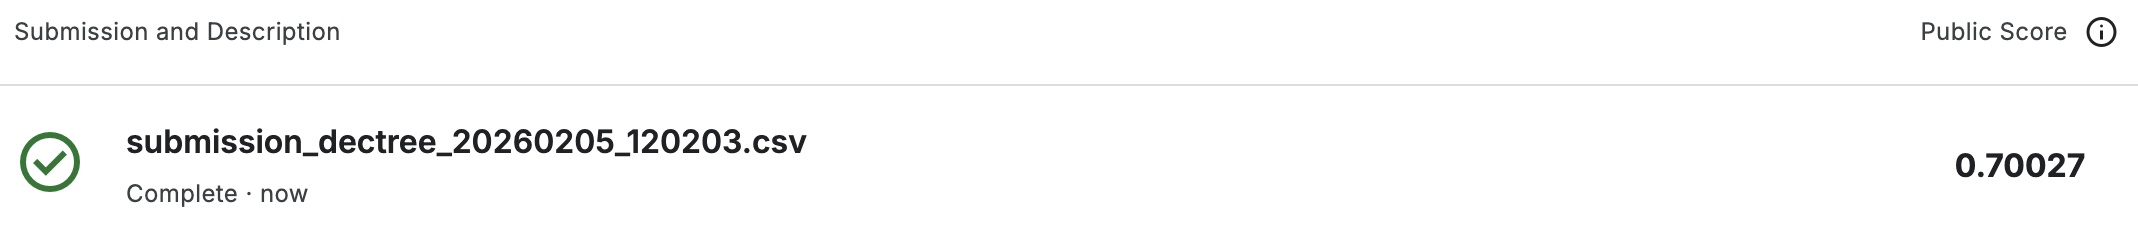
\includegraphics[width=0.85\linewidth]{./figs/dectree_2026-02-05_12-03-06.png}
    \caption{决策树的实验结果}
    \label{fig:enhancement-dectree}
\end{figure}



\subsubsection{贝叶斯方法}
我们采用朴素贝叶斯作为本次实验中贝叶斯方法的代表进行测试。朴素贝叶斯不涉及超参数的配置。TF-IDF 最大特征数为 5000，n-gram 范围为 $(1,1)$。实验结果如图~\ref{fig:enhancement-nb} 所示。

\begin{figure}[H]
    \centering
    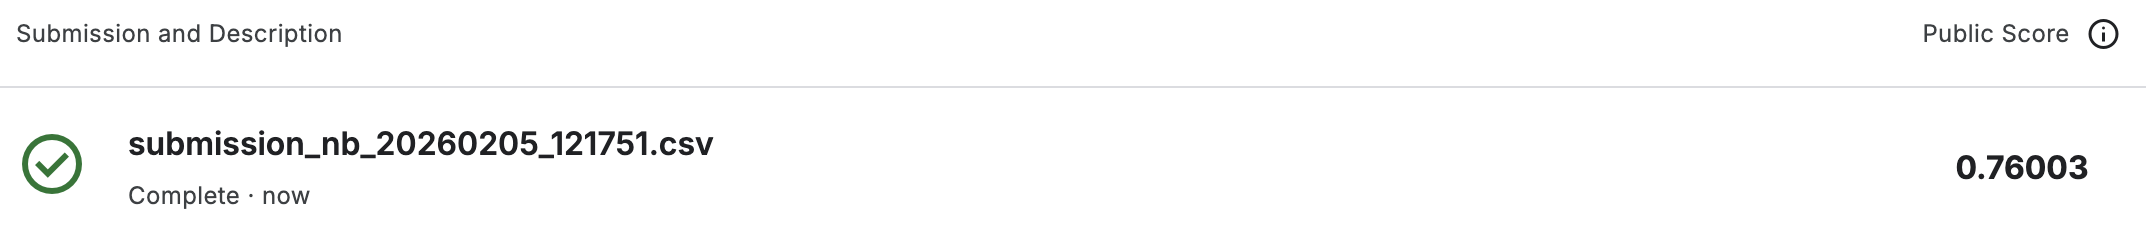
\includegraphics[width=0.85\linewidth]{./figs/nb_2026-02-05_12-18-37.png}
    \caption{朴素贝叶斯的实验结果}
    \label{fig:enhancement-nb}
\end{figure}

朴素贝叶斯分类器取得了 0.76003 的F1分数，其性能介于决策树与线性模型之间。该模型基于生成模型假设以及特征条件独立的强假设，计算效率极高。在文本的「词袋」表示下，这一假设虽与实际不符，却往往能产生令人惊讶的基线效果。然而，也正是由于忽略了特征间的相关性，其建模能力存在理论上限，无法像逻辑回归或支持向量机那样通过数据驱动的方式学习更优的特征权重组合，因此其性能被更强大的线性模型所超越。



\section{BERT}
BERT（Bidirectional Encoder Representations from Transformers）是 Google 于 2018 年提出的一种基于 Transformer Encoder 的预训练语言模型~\cite{BERT}。其核心创新在于采用\textbf{双向上下文理解}机制，通过掩码语言模型（Masked Language Model, MLM）和下一句预测（Next Sentence Prediction, NSP）两个任务进行预训练，从而能够更好地捕捉句子内部和句子间的语义关系。

BERT 模型的结构基于多层 Transformer 编码器堆叠而成，通过在大规模语料上进行预训练后，可以针对下游任务进行微调。BERT 支持多种自然语言处理任务，包括文本分类、句子对匹配、序列标注和问答等，其统一的结构设计使得模型具有很强的迁移学习能力。这种迁移学习范式极大减少了下游任务对标注数据规模的依赖，非常适合本项目中规模较小的灾难推文数据集。



\subsection{设计思路}
BERT（Bidirectional Encoder Representations from Transformers）的核心设计思路在于通过预训练深度双向 Transformer 编码器来学习通用语言表示，从而在下游任务中进行微调。传统语言模型通常采用单向或浅层双向结构，而 BERT 通过掩码语言模型（Masked Language Model, MLM）和下一句预测（Next Sentence Prediction, NSP）任务，实现了对上下文信息的深层双向建模。其设计遵循"预训练-微调"范式，通过在大量无标签文本上进行预训练，捕捉词汇、句法和语义层面的特征，再针对具体任务进行有监督微调。



\subsection{模型架构}
\subsubsection{Transformer Encoder 结构}\label{sec:bert-arch-transformer}
BERT 的基础结构来源于 Transformer Encoder，其核心组件为 Multi-Head Self-Attention 多头自注意力机制和 Feed Forward Network 前馈神经网络。对于输入序列 $X = \{x_1, x_2, \ldots, x_n\}$，首先映射为词向量表示：
\begin{equation}
H^{(0)} = \text{Embedding}(X) + \text{PositionEncoding}
\end{equation}

其中包含，token 嵌入、segment 嵌入、position 嵌入，序列开头加入特殊符号 \verb|[CLS]|，其输出向量用于分类任务。在每一层 Encoder 中，输入通过多头注意力机制：

\begin{equation}
\text{Attention}(Q,K,V) = \text{softmax}\left(\dfrac{\displaystyle QK^{\top}}{\displaystyle\sqrt{d_k}}\right)V
\end{equation}

其中，$Q$(uery) 为查询矩阵、$K$(ey) 为键矩阵、$V$alue 为值矩阵，$d_k$ 为词嵌入向量维度。多头注意力的计算为：

\begin{equation}
\text{MultiHead}(Q,K,V) = \text{Concat}(\text{head}_1,\text{head}_2,\ldots,\text{head}_h)W^O
\end{equation}

随后进入前馈网络：
\begin{equation}
\text{FFN}(x) = \max(0, xW_1 + b_1)W_2 + b_2
\end{equation}

每层均包含残差连接与 Layer Normalization 归一化层：
\begin{equation}
\text{LayerNorm}\left[x + \text{Sublayer}(x)\right]
\end{equation}



\subsubsection{BERT 结构}
设 BERT 中所使用的 Transformer 编码器层数为 $L$，隐藏层维度为 $H$，自注意力头数为 $A$，则模型参数总量约为 $O(L \times H^2)$。

\textbf{模型结构示意图解析：} 如图\ref{fig:bert_tasks}所示，BERT 采用统一的编码器架构支持多种下游任务：
\begin{itemize}
    \item \textbf{句子对分类任务（图a）}：输入为两个句子，以 [SEP] 标记分隔，起始位置添加 [CLS] 标记。编码器输出中，[CLS] 位置的隐藏状态用于分类任务（如 MNLI、QQP、QNLI、SST-B、MRPC）。
    \item \textbf{单句分类任务（图b）}：输入为单个句子，起始位置添加 [CLS] 标记。[CLS] 位置的隐藏状态用于分类任务（如 SST-2、CoLA）。
    \item \textbf{问答任务（图c）}：输入为问题和段落的拼接，以 [SEP] 分隔。模型需要预测答案在段落中的起始和结束位置（如 SQuAD v1.1），通过输出序列中每个位置的概率分布实现。
    \item \textbf{序列标注任务（图d）}：输入为单个句子，每个标记对应的隐藏状态用于标记预测（如 CoNLL-2003 NER），实现词级别的分类任务。
\end{itemize}

\begin{figure}[htbp]
    \centering
    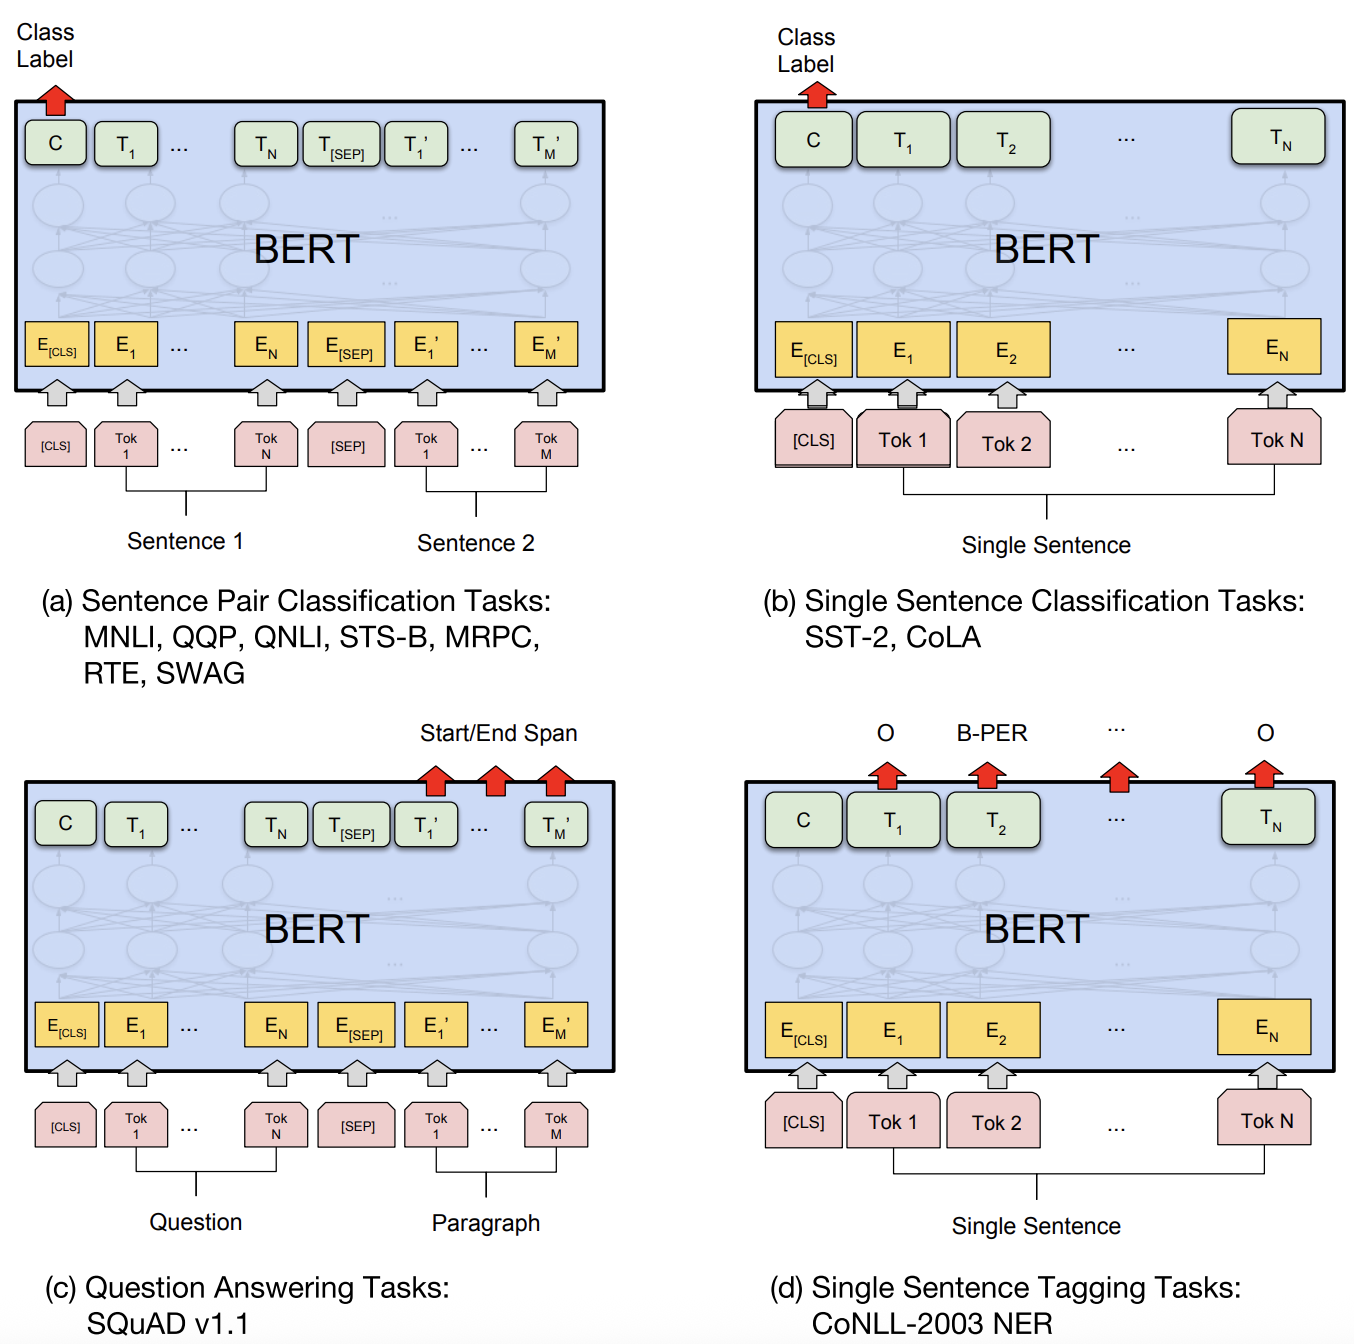
\includegraphics[width=0.95\textwidth]{./figs/bert-structure.png}
    \caption{BERT 在不同任务中的应用架构示意图：(a) 句子对分类任务，(b) 单句分类任务，(c) 问答任务，(d) 序列标注任务。图中展示了输入格式、特殊标记的使用方式以及输出层的设计差异。}
    \label{fig:bert_tasks}
\end{figure}

模型通过多层自注意力机制与前馈神经网络进行特征变换，每一层的计算可表示为：
\[
\mathbf{H}^{(l)} = \text{TransformerBlock}(\mathbf{H}^{(l-1)}), \quad l = 1, \dots, L
\]
其中 $\mathbf{H}^{(0)}$ 与 \ref{sec:bert-arch-transformer} 中含义相同，
% $\mathbf{H}^{(0)} = \mathbf{E}(\mathbf{X})$，
$\mathbf{H}^{(L)}$ 为最后一层输出。不同任务仅在输出层设计上有所差异，体现了 BERT 架构的统一性和灵活性。



\subsection{优化与损失函数}
BERT 的预训练阶段通过两个任务联合优化模型参数：掩码语言模型（MLM）和下一句预测（NSP）。MLM 任务随机掩盖输入中 15\% 的标记，并预测被掩盖的原始标记。设掩盖后的输入为 $\tilde{\mathbf{X}}$，掩盖位置集合为 $\mathcal{M}$，则 MLM 损失为：
\[
\mathcal{L}_{\text{MLM}} = -\sum_{i \in \mathcal{M}} \log P(x_i \mid \tilde{\mathbf{X}})
\]
其中 $P(x_i \mid \tilde{\mathbf{X}})$ 通过 softmax 函数计算。NSP 任务用于学习句子间关系，给定两个句子 A 和 B，模型预测 B 是否为 A 的下一句，损失函数为二元交叉熵：
\[
\mathcal{L}_{\text{NSP}} = -\log P(y \mid \mathbf{X}_{A}, \mathbf{X}_{B})
\]
总预训练损失为两者之和：
\[
\mathcal{L}_{\text{pretrain}} = \mathcal{L}_{\text{MLM}} + \mathcal{L}_{\text{NSP}}
\]
在微调阶段，根据下游任务的不同，在 BERT 输出之上添加任务特定的分类层或序列标注层，并采用对应的监督损失（如交叉熵损失）进行端到端优化。

譬如，在本实验中所进行的文本分类任务中，取最后一层 \verb|[CLS]| 向量作为句子表示 $h = H_{\verb|[CLS]|}$，并通过全连接层进行分类 $y = \text{softmax}(Wh + b)$，最后用交叉熵损失函数 $\mathcal{L} = - \displaystyle\sum y \log \hat{y}$ 优化。交叉熵损失函数的展开介绍见 \ref{sec:adab-bert-loss}~节。

与传统的 TF-IDF 或 n-gram 方法相比，BERT 在本任务中具有明显优势，它能处理语义歧义词汇，譬如 fire、explosion，它能够理解上下文关系而非单词频率，对短文本具有较强表示能力，并且能利用预训练知识弥补数据规模不足。此外，我们小组通过将 keyword 和 location 信息拼接进入输入文本，使 BERT 在统一语义空间中学习结构化特征与文本特征之间的关联，进一步提升分类效果。



\subsection{实验结果}
设定的训练迭代为 64 次，学习率为 2e-5，批次数为 192 个样本量，最大序列长度为 128 个 token，训练设备为 A6000 NVIDIA CUDA GPU。一共设置四个参数组，分别得到不同测试集的最终 Kaggle 得分，其中对照组是直接将 Twitter 内容直接用于 BERT 中文模型（bert-base-chinese）训练，另外三组分别是 BERT 英文模型（bert-large-uncased）直接训练、BERT 中文模型训练处理后的数据集、BERT 英文模型训练处理后的数据集。历史记录见\autoref{fig-history} 所示，Kaggle 的 BERT 模型最高分排名见\autoref{fig-bert-rank} 所示，得分增长幅度见\autoref{tab-increase} 所示。

\begin{table}[H]
    \centering
    \setlength{\tabcolsep}{12pt}
    \renewcommand{\arraystretch}{1.5}
    \caption{BERT 在不同预训练模型和数据集下的结果}\label{tab-increase}
    \begin{tabular}{clccc}
        \bottomrule[1.5pt]
        \@ & \textbf{模型} & \textbf{参数} & \textbf{得分} & \textbf{增率} \\
        \midrule[0.5pt]
        \rowcolor{MorandiLightCyan}\cube{MorandiBlue} & bert-base-chinese & 原始数据集 & 0.77352 & - \\
        \cube{MorandiGrey} & bert-large-uncased & 原始数据集 & 0.82470 & $\bm{6.62\%\uparrow}$ \\
        \cube{MorandiOrange} & bert-base-chinese & 处理后的数据集 & 0.83052 & $\bm{7.37\%\uparrow}$ \\
        \cube{MorandiRed} & bert-large-uncased & 处理后的数据集 & 0.83879 & $\bm{8.44\%\uparrow}$ \\
        \toprule[1.5pt]
    \end{tabular}
\end{table}



\begin{figure}[H]
    \centering
    \includegraphics*[scale=0.35]{./figs/BERT-History.png}
    \caption{BERT 得分历史}\label{fig-history}
\end{figure}


\begin{figure}[H]
    \centering
    \includegraphics*[scale=0.25]{./figs/BERT-Rank.png}
    \caption{BERT 最高得分（第 79 名前 15\%）}\label{fig-bert-rank}
\end{figure}



\section{AdaBoost 集成}
\subsection{Boosting 算法以及 AdaBoost 介绍}

Boosting 算法是一种将多个学习器集成为一个模型的算法。具体而言，其通过串行地训练多个学习器，使得其中每个都针对前一个模型改进。其能够减小模型的偏差，但对方差影响不大。在集成时，一般使用简单模型（偏差小、方差大）作为基学习器集成，最终使用所有基学习器的加权和或投票结果作为预测结果。

AdaBoost 是 Boosting 算法中的代表之一。该算法通过在串行训练每个学习器的期间不断调整训练数据点的权重，增大当前一轮学习器分类错误样本的权重、减小当前一轮学习器分类正确样本的权重，最终使得后面的学习器能够愈发关注于此前学习器分类错误的样本，逐渐迭代改善所有学习器整体的性能。在最终预测的时候，算法会根据每个学习器训练期间的错误率确定一个权重值，并将每个学习器的加权预测结果作为输出。

具体而言，AdaBoost 的算法流程可以总结如下。在下方的形式化表述中，本文使用 $h_t(\boldsymbol{x}): \mathbb{R}^d \mapsto \{ -1, 1\}$ 表示第 $t$ 轮训练（第 $t$ 个学习器）；$D_t (i)$ 表示第 $t$ 轮训练所使用的训练集权重，括号内的 $i$ 表示第 $i$ 个训练数据；$N$ 表示训练集样本点数目；$T$ 表示总训练轮数（基学习器数目）。

\textit{
\begin{enumerate}
    \item 给定训练数据 $\{(\boldsymbol{x}_1, y_1), (\boldsymbol{x}_2, y_2), \cdots, (\boldsymbol{x}_N, y_N)\}$；
    \item 初始化第一轮的训练数据权重 $D_1=\{1/N, 1/N, \cdots, 1/N\}$；
    \item 迭代训练 $t \in \{1, 2, \cdots, T\}$：
    \begin{enumerate}
        \item 使用权重 $D_t$ 来训练学习器 $h_t(\boldsymbol{x})$；
        \item 计算学习器 $h_t$ 在训练集上的错误率 $\epsilon_t$：
        $$\epsilon_t=\sum_{i=1}^{N}D_t(i) \cdot \mathbb{I}[h_t(\boldsymbol{x}_i)\ne y_i]$$
        \item 计算学习器 $h_t$ 的预测权重 $\alpha_t$：
        $$\alpha_t = \frac12 \ln \left( \frac{1-\epsilon_t}{\epsilon_t} \right)$$
        \item 更新训练数据权重 $D_{t+1}$（下式中 $Z_{t+1}$ 为归一化因子）：
        $$D_{t+1}(i) = \frac{D_t(i)}{Z_{t+1}} \cdot \exp \{-\alpha_t y_i h(\boldsymbol{x}_i)\}$$
        \item 进入下一轮迭代。
    \end{enumerate}
    \item 训练好所有的学习器之后，最终预测结果为：
    $$\hat y = \mathrm{sign}\left[\sum_{t=1}^T \alpha_t h_t(\boldsymbol{x})\right]$$
\end{enumerate}
}

在上述迭代训练过程中，每一轮训练基学习器 $h_t$ 需要使用训练样本权重 $D_t$。此处可以直接集成到基学习器训练期间的损失函数中实现。比如定义单样本的损失值为 $l(\hat{y}_i, y_i)$，某次训练的总损失为 $\mathcal{L}(\theta)=\sum_{i=1}^N l(\hat{y}_i, y_i)$，那么可以使用下述损失函数实现对训练数据的加权：
$$\mathcal{L}(\theta)=\sum_{i=1}^N D_t(i) \cdot l(\hat{y}_i, y_i)$$

在 AdaBoost 中，随着训练轮数（学习器数目）的增加，误差具有理论上严格递减的上界：
$$\frac{1}{N} \sum_{i=1}^N \mathbb{I}(\hat{y}_i \ne y_i) \le \exp \left\{ -2 \sum_{t=1}^T \left(\frac{1}{2} -\epsilon_t \right)^2 \right\}$$
此处假定其中每一个学习器的误差 $\epsilon_t < 0.5$，也就是「无论学习器有多差，都得好于随机猜测（后者为 0.5 的错误率）」。另外，如果某个学习器有 $\epsilon_t > 0.5$，那么只需要将其预测标签翻转即可实现 $\epsilon_t < 0.5$。故而，理论上而言，使用 AdaBoost 可以随着基学习器的数目增多而逐渐增加模型整体的性能。

\subsection{与 BERT 分类器的结合}

BERT 分类器由一个 BERT 模型作为特征提取器，另加下游的一个线性层（全连接层）连接而成。其中线性层用于将 BERT 提取出的特征维度映射到类别维度。如一个二分类问题，该线性层负责将 $D$ 维的 BERT 特征映射到 2 维，形成针对两个类别的 logit 分数。

\subsubsection{损失函数实现}
\label{sec:adab-bert-loss}

在标准的 BERT 分类器微调过程中，最常见的做法是针对各类别的 logit 分数与正确标签使用交叉熵损失作为损失函数。对于 $K$ 分类问题，记 $N$ 个样本形成的 logits 为 $\mathbf{S} \in \mathbb{R}^{N\times K}$，第 $i$ 个样本的 logit 为 $\boldsymbol{s}_{i} \in \mathbb{R}^{K}$，即 $\mathbf{S}$ 的第 $i$ 个行向量，交叉熵损失定义如下：
$$
- \sum_{i=1}^{N} \sum_{k=1}^{K} \mathbb{I}(y_{i}=k) \cdot \log (\mathrm{softmax}(\boldsymbol{s}_{i})^{(k)})
$$
其中 $\mathrm{softmax}(\boldsymbol{s}_{i})^{(k)}$ 为向量 $\boldsymbol{s}_{i}$ 经过 softmax 运算之后的第 $k$ 维分量值。上述过程可以使用下述 PyTorch 风格的伪代码表示：

% \lstset{
%  columns=fixed,       
%  numbers=left,                                        % 在左侧显示行号
%  numberstyle=\tiny\color{gray},                       % 设定行号格式
%  frame=none,                                          % 不显示背景边框
%  backgroundcolor=\color[RGB]{245,245,244},            % 设定背景颜色
%  keywordstyle=\color[RGB]{40,40,255},                 % 设定关键字颜色
%  numberstyle=\footnotesize\color{darkgray},           
%  commentstyle=\it\color[RGB]{0,96,96},                % 设置代码注释的格式
%  stringstyle=\rmfamily\slshape\color[RGB]{128,0,0},   % 设置字符串格式
%  showstringspaces=false,                              % 不显示字符串中的空格
%  language=Python,                                        % 设置语言
% }

\begin{small}
\begin{lstlisting}[language=Python]
# Given logit matrix S shaped [N, K],
# and ground-truth labels y_gt shaped [K]:
lls  = torch.log_softmax(S, dim=1)  # log likelihood
loss = torch.nn.functional.nll_loss(
    lls, y_gt,
    reduction='mean'
)
\end{lstlisting}
\end{small}

即：

\begin{small}
\begin{lstlisting}[language=Python]
loss = torch.nn.CrossEntropyLoss()(S, y_gt)
\end{lstlisting}
\end{small}

使用按步骤拆分后的交叉熵损失后，此时可以引入每个样本点的权重。首先可以将交叉熵损失的定义式稍作修改如下：
$$
- \sum_{i=1}^{N} D(i) \cdot \left[ \sum_{k=1}^{K} \mathbb{I}(y_{i}=k) \cdot \log (\mathrm{softmax}(\boldsymbol{s}_{i})^{(k)}) \right]
$$
上式中 $D(i)$ 即对应第 $i$ 个样本点的权重值；并且 $D$ 满足 $\sum_{i=1}^{N}D(i)=1$。

根据上式修改，此时可以将交叉熵损失的伪代码改写如下：

\begin{small}
\begin{lstlisting}[language=Python]
# Given S, y_gt and
# sample weight vector D shaped [N] s.t. sum(D)=1
lls     = torch.log_softmax(S, dim=1)
weights = D.expand(K, -1).T
w_lls   = lls * weights
loss    = torch.nn.functional.nll_loss(
    w_lls, y_gt,
    reduction='sum'
)
\end{lstlisting}
\end{small}

其中 \verb|weights| 变量为经过复制、扩展之后的 $D$ 向量。如给定 $D=(0.1, 0.2, 0.7)^{\top}$，并且 $K=2$，那么最终有
$$
\mathrm{weights}= \left[\begin{matrix}
0.1 & 0.1 \\
0.2 & 0.2 \\
0.7 & 0.7
\end{matrix}\right]
$$
另外也需要注意，由于我们显式地为似然值施加了权重（\verb|w_lls = lls * weights|），所以在最终的 \verb|nll_loss| 函数中应声明 \verb|reduction='sum'|。

\subsubsection{小批次训练}
\label{sec:adab-bert-minibatch}

由于常见的语言模型训练集都超过了数千个样本（如本题目中提供的训练集样本点数为约 7000 个），所以一般不能够直接将所有样本合并为单独一个批次交由 BERT 分类器训练，需要拆分为更小的 batch，如 $n$ 个样本一个 batch（$n\ll N$）。

在拆分至更小的 batch 之后，此时前文中提到的训练集样本点权重向量 $D$ 不能够再直接拿来使用，需要先从中拆分出对应每个小 batch 的 $n$ 维权重数据 $d \in \mathbb{R}^{n}$。同时，为了使得模型能够在每个小 batch 上更新梯度，即使得每个小 batch 的损失函数值保持与全局损失函数语义上的一致性，我们采取了对向量 $d$ 再次进行一次归一化操作的方案。

经过上述处理，此时的小 batch 交叉熵损失可以定义如下：
$$
- \frac{1}{Z}\sum_{i=i_{0}}^{i_{0}+n} D(i) \cdot \left[ \sum_{k=1}^{K} \mathbb{I}(y_{i}=k) \cdot \log (\mathrm{softmax}(\boldsymbol{s}_{i})^{(k)}) \right]
$$
其中 $i_{0}$ 为该小 batch 的样本下标初始值，$Z$ 为针对 $D(i)$ 的归一化因子，定义为 $Z=\sum_{i=i_{0}}^{i_{0}+n} D(i)$。最终有 $d(i)=D(i)/Z$。

对应的伪代码即：

\begin{small}
\begin{lstlisting}[language=Python]
# Given D
for i0 in batch_begin_indices:
    j = min(N, i0 + n)
    d = D[i0, j] / sum(D[i0, j])
    # ... (procedure to get batch logit matrix S shaped [n, K])
    lls     = torch.log_softmax(S, dim=1)
    weights = d.expand(K, -1).T
    w_lls   = lls * weights
    loss    = torch.nn.functional.nll_loss(
        w_lls, y_gt,
        reduction='sum'
    )
\end{lstlisting}
\end{small}

经过上述 \ref{sec:adab-bert-loss}~节和 \ref{sec:adab-bert-minibatch}~节两个步骤，便定义了 AdaBoost + BERT 的损失函数与训练方法。

\subsection{代码实现}

鉴于版面有限，本节仅节选具体实现 AdaBoost + BERT 的核心逻辑的代码。

\subsubsection{AdaBoost 参数更新}

\begin{small}
\begin{lstlisting}[language=Python]
def inner_train_adaboost(model, train_loader, stage):
    ## Train the model
    optimizer = torch.optim.AdamW(
        model.parameters(),
        lr = LEARNING_RATE
    )
    model = _inner_training_loop(
        model=model,
        optimizer=optimizer,
        train_loader=train_loader,
        model_id=stage,
    )

    ## Update AdaBoost parameters
    model.eval()
    # 1. Keep track of train error (epsilon_t)
    train_error = 0
    train_predictions = []
    train_labels = []
    train_sample_indices = []
    with torch.no_grad():
        for batch in train_loader:
            input_ids       = batch['input_ids']
            attention_mask  = batch['attention_mask']
            labels          = batch['labels']
            weights         = batch['weights']
            sample_indices  = batch['idx']
            
            outputs = model.forward(
                input_ids,
                attention_mask=attention_mask
            )
            _, predictions = torch.max(outputs.logits, dim=1)

            train_predictions.append(predictions)
            train_labels.append(labels)
            train_sample_indices.append(sample_indices)

            train_error += weights[predictions != labels].sum()

    y_preds = torch.cat(train_predictions, dim=0)
    y_gts   = torch.cat(train_labels, dim=0)
    indices = torch.cat(train_sample_indices, dim=0)

    # 2. Get current model weight (alpha_t)
    alpha = 0.5 * torch.log((1 - train_error) / train_error)

    # 3. Update dataset weights (D_t)
    weight_factors = torch.full_like(y_preds, alpha)
    weight_factors = torch.masked_fill(
        weight_factors,
        y_preds == y_gts,
        -alpha
    )
    weight_factors = torch.exp(weight_factors)

    for i in range(len(train_loader.dataset)):
        sample_idx = indices[i]
        weight_factor = weight_factors[i]
        data_weights[sample_idx] *= weight_factor
    data_weights /= sum(data_weights)
\end{lstlisting}
\end{small}

上述函数在具体使用时，串行初始化各个模型作为 \verb|model| 参数的输入，并且在不同的模型上使用同一组训练数据加载器 \verb|train_loader|，最终标明每个模型在训练时的序号输入 \verb|stage| 即可。另外，函数中尚未定义的 \verb|_inner_training_loop| 方法将在 \ref{sec:adab-code-training}~节中给出。

\subsubsection{BERT 训练}
\label{sec:adab-code-training}

\begin{small}
\begin{lstlisting}[language=Python]
def _inner_training_loop(
    model,optimizer,
    train_loader, model_id
):
    for epoch in range(EPOCHS):
        model.train()
        for idx, batch in enumerate(train_loader):
            input_ids       = batch['input_ids']
            attention_mask  = batch['attention_mask']
            labels          = batch['labels']
            weights         = batch['weights']

            optimizer.zero_grad()
            outputs = model.forward(
                input_ids,
                attention_mask=attention_mask,
                labels=labels
            )
            
            # loss = outputs.loss
            logits  = outputs.logits
            lls     = torch.log_softmax(logits, dim=-1)
            weights = weights / weights.sum()
            w_lls   = torch.stack([weights, weights], dim=0).T * lls
            loss    = torch.nn.functional.nll_loss(
                w_lls, labels,
                reduction='sum'
            )

            loss.backward()
            optimizer.step()
        # Here keep a best copy of trained model...
    return model
\end{lstlisting}
\end{small}

可以看到，在具体的代码实现中，我们将每个样本点的权重值设置为了数据集的一个成员，在数据加载器（\verb|DataLoader|）采样数据时伴随着返回，得到上述代码中的 \verb|weights| 变量。另外，代码中的 \verb|torch.stack([weights, weights], dim=0).T| 与前文中对应的 \verb|weights.expand(2, -1).T| 等价。



\subsection{实验结果}
本次实验使用了 5 个 BERT 分类器使用 AdaBoost 集成的结果，其中每个 BERT 分类器训练 10 个 epoch。最终得到的每个分类器的错误率（$\epsilon_t$）以及权重（$\alpha_t$）分别为 $(7.81\%, 28.54\%, 45.00\%, 5.74\%, 24.63\%)$ 和 $(1.2343, 0.4589, 0.1002, 1.3992,0.5591)$。如图~\ref{fig:adab-result} 所示，最终在测试集上的结果于 Kaggle 平台上得分 0.8421 分，于报告书写时（\date{\today}）位列第 49/563 名，属前 10\%，证实了 AdaBoost 的有效性。

\begin{figure}[H]
    \centering
    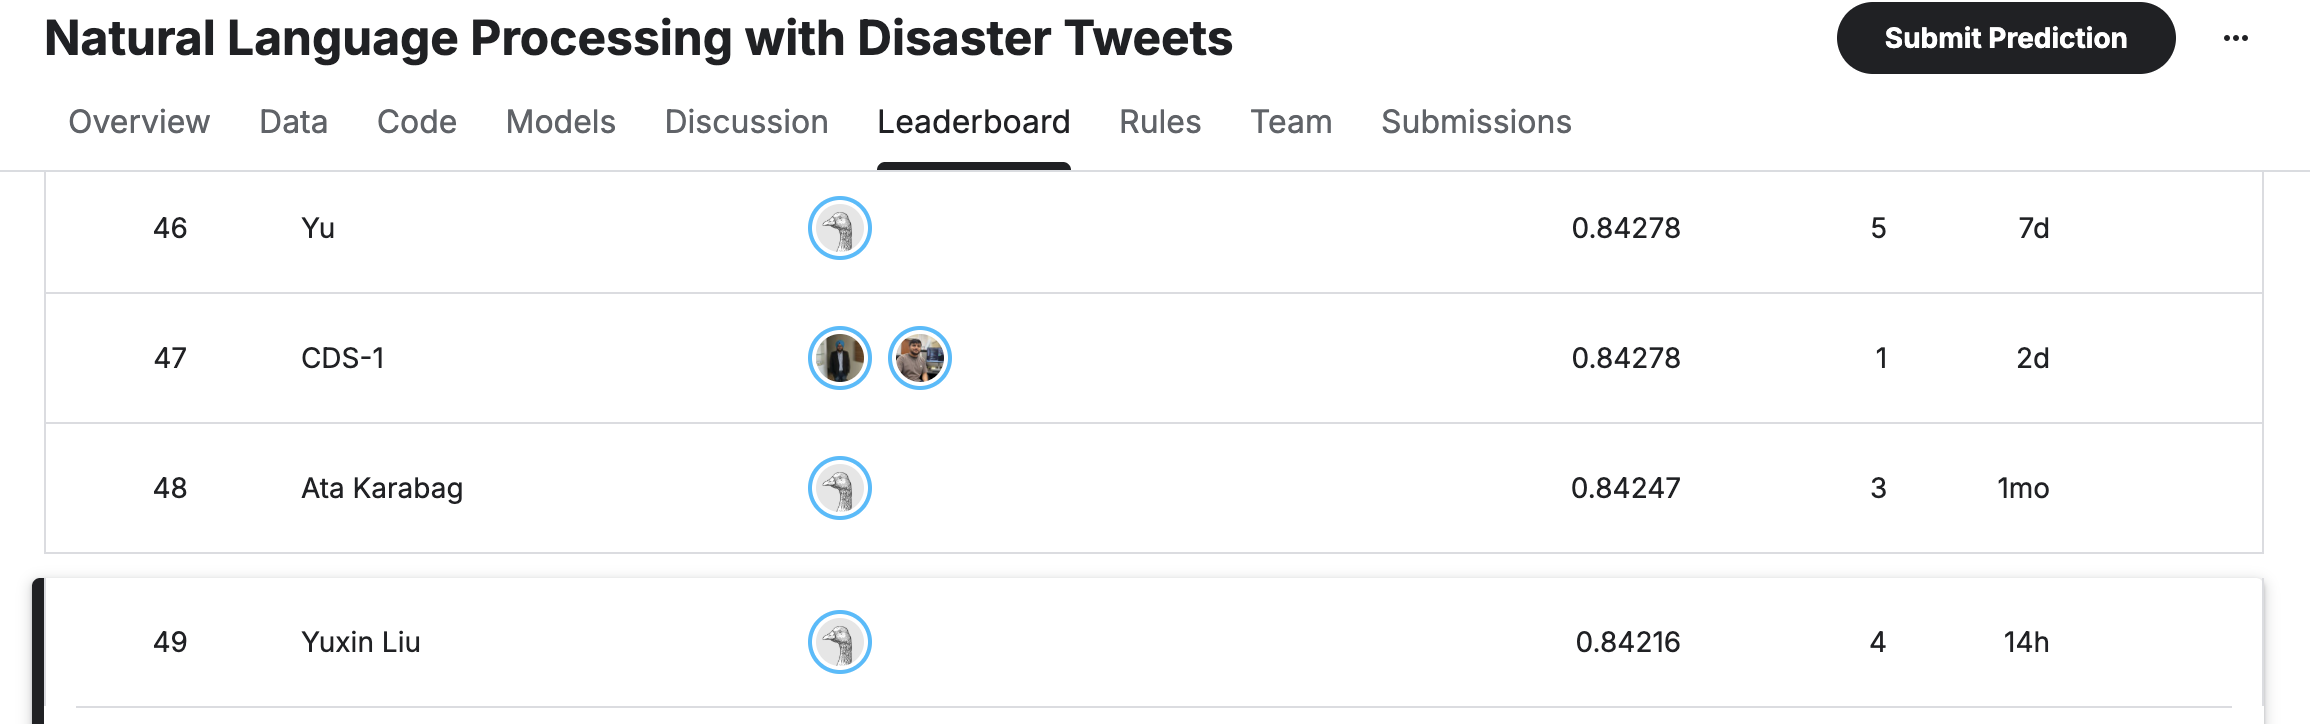
\includegraphics[width=0.85\linewidth]{./figs/adaboost_result.png}
    
\includegraphics[width=0.85\linewidth]{./figs/adaboost_result_rank.png}
    \caption{AdaBoost + BERT 方法在 Kaggle 上的测试结果}
    \label{fig:adab-result}
\end{figure}



\section{分工介绍}
\begin{itemize}
    \item \textbf{刘X}：撰写 SVM、决策树、贝叶斯等机器学习模型原理，对 BERT 原理进行完善
    \item \textbf{刘XX}：撰写 AdaBoost 集成学习部分、编程 Baseline 逻辑回归、SVM、决策树、AdaBoost 相关代码
    \item \textbf{Illusionna}：撰写竞赛背景、进行数据探索性分析、数据预处理、通过不同参数组逐步提高 BERT 模型得分
\end{itemize}






\reference



\end{document}